%
%	Configure LaTeX to produce a PDF presentation using the beamer class
%

\documentclass[ignorenonframetext,11pt]{beamer}
\usepackage[ngerman]{babel}
\usepackage[utf8]{inputenc}		% For UTF-8 support
\usepackage[T1]{fontenc}

\usepackage{graphicx}


\usepackage{beamerthemesplit}
\usepackage{patchcmd}
\usepackage{tabulary}		% Support longer table cells
\usepackage{booktabs}		% Support better tables
\usepackage[sort&compress]{natbib}

\usepackage{framed}			% Allow background color for images
\definecolor{shadecolor}{named}{white}


\usepackage{subfigure}

\let\oldSubtitle\subtitle


% Configure default metadata
\input{mmd-default-metadata}


%\AtBeginSection[]
%{
 %\begin{frame}
    %\frametitle{Inhalt}
	%\tableofcontents %[currentsection,currentsubsection]
   %\end{frame}
%}


\long\def\citefoot#1{\let\thefootnote\relax\footnotetext{\citet{#1}} }

\def\mytitle{File Network: Fortschrittsberichte}
\def\myauthor{Anastasia Kazakova, Bengt Lüers}
\def\latexmode{beamer}
\def\latexxslt{beamer}
\def\theme{keynote-IntSysTheme}
\input{mmd-natbib-plain}
\def\bibliocommand{\bibliography{Literaturliste}}
\def\bibliostyle{chicago}
%
%	Get ready for the actual document
%

%
% Use default MMD metadata for beamer equivalents
%

\ifx\subtitle\undefined
\else
	\oldSubtitle{\subtitle}
\fi

\ifx\affiliation\undefined
\else
	\institute{\affiliation}
\fi

\ifx\mydate\undefined
	\def\mydate{\today}
\else
	\date{\mydate}
\fi

\ifx\event\undefined
\else
	\date[\mydate]{\mydate~ / \event }
\fi


%\input{mmd-title}

% Show "current/total" slide counter in footer
\title[\mytitle\hspace{2em}\insertframenumber/
\inserttotalframenumber]{\mytitle}


\author{\myauthor}
\addtolength{\parskip}{\baselineskip}

\ifx\theme\undefined
\else
	\usetheme{\theme}
\fi

\begin{document}
\frame[plain]{\setlength\parskip{0pt}\titlepage}

\# \#

\section{Listen}
\label{listen}

\begin{frame}

\frametitle{Nummerierte Liste}
\label{nummerierteliste}

\begin{enumerate}
\item \textbf{Ich bin}

\item eine nummerierte Liste

\item mit drei Punkten

\end{enumerate}

\end{frame}

\begin{frame}

\frametitle{Einfache Liste}
\label{einfacheliste}

\begin{itemize}
\item Ich bin

\item eine einfache Liste

\item mit drei Punkten

\begin{itemize}
\item und eins

\item zwei Unterpunkten

\end{itemize}

\end{itemize}

\end{frame}

\section{Textformatierung}
\label{textformatierung}

\begin{frame}

\frametitle{Blockzitat}
\label{blockzitat}

\begin{quote}

Lorem ipsum dolor sit amet, consetetur sadipscing elitr, sed diam nonumy eirmod tempor invidunt ut labore et dolore magna aliquyam erat, sed diam voluptua. At vero eos et accusam et justo duo dolores et ea rebum. Stet clita kasd gubergren, no sea takimata sanctus est Lorem ipsum dolor sit amet.
\end{quote}

\end{frame}

\begin{frame}

\frametitle{Wenn es mal schräg und dick sein darf}
\label{wennesmalschrgunddickseindarf}

Ich bin \textbf{dick}

Und ich bin \emph{schräg}

\end{frame}

\section{Zitieren}
\label{zitieren}

\begin{frame}

\frametitle{Ohne Bibtex}
\label{ohnebibtex}

Wenn man was mal zitieren möchte ~\citep{Doe}.

Oder mal was anders ~\citep{Johnson}.

\end{frame}

\begin{frame}

\frametitle{Mit Bibtex}
\label{mitbibtex}

Ich zitiere auch ~\citep{Wickens}.

\end{frame}

\section{Bilder und Tabellen}
\label{bilderundtabellen}

\begin{frame}

\frametitle{Bild}
\label{bild}

\begin{figure}[htbp]
\centering
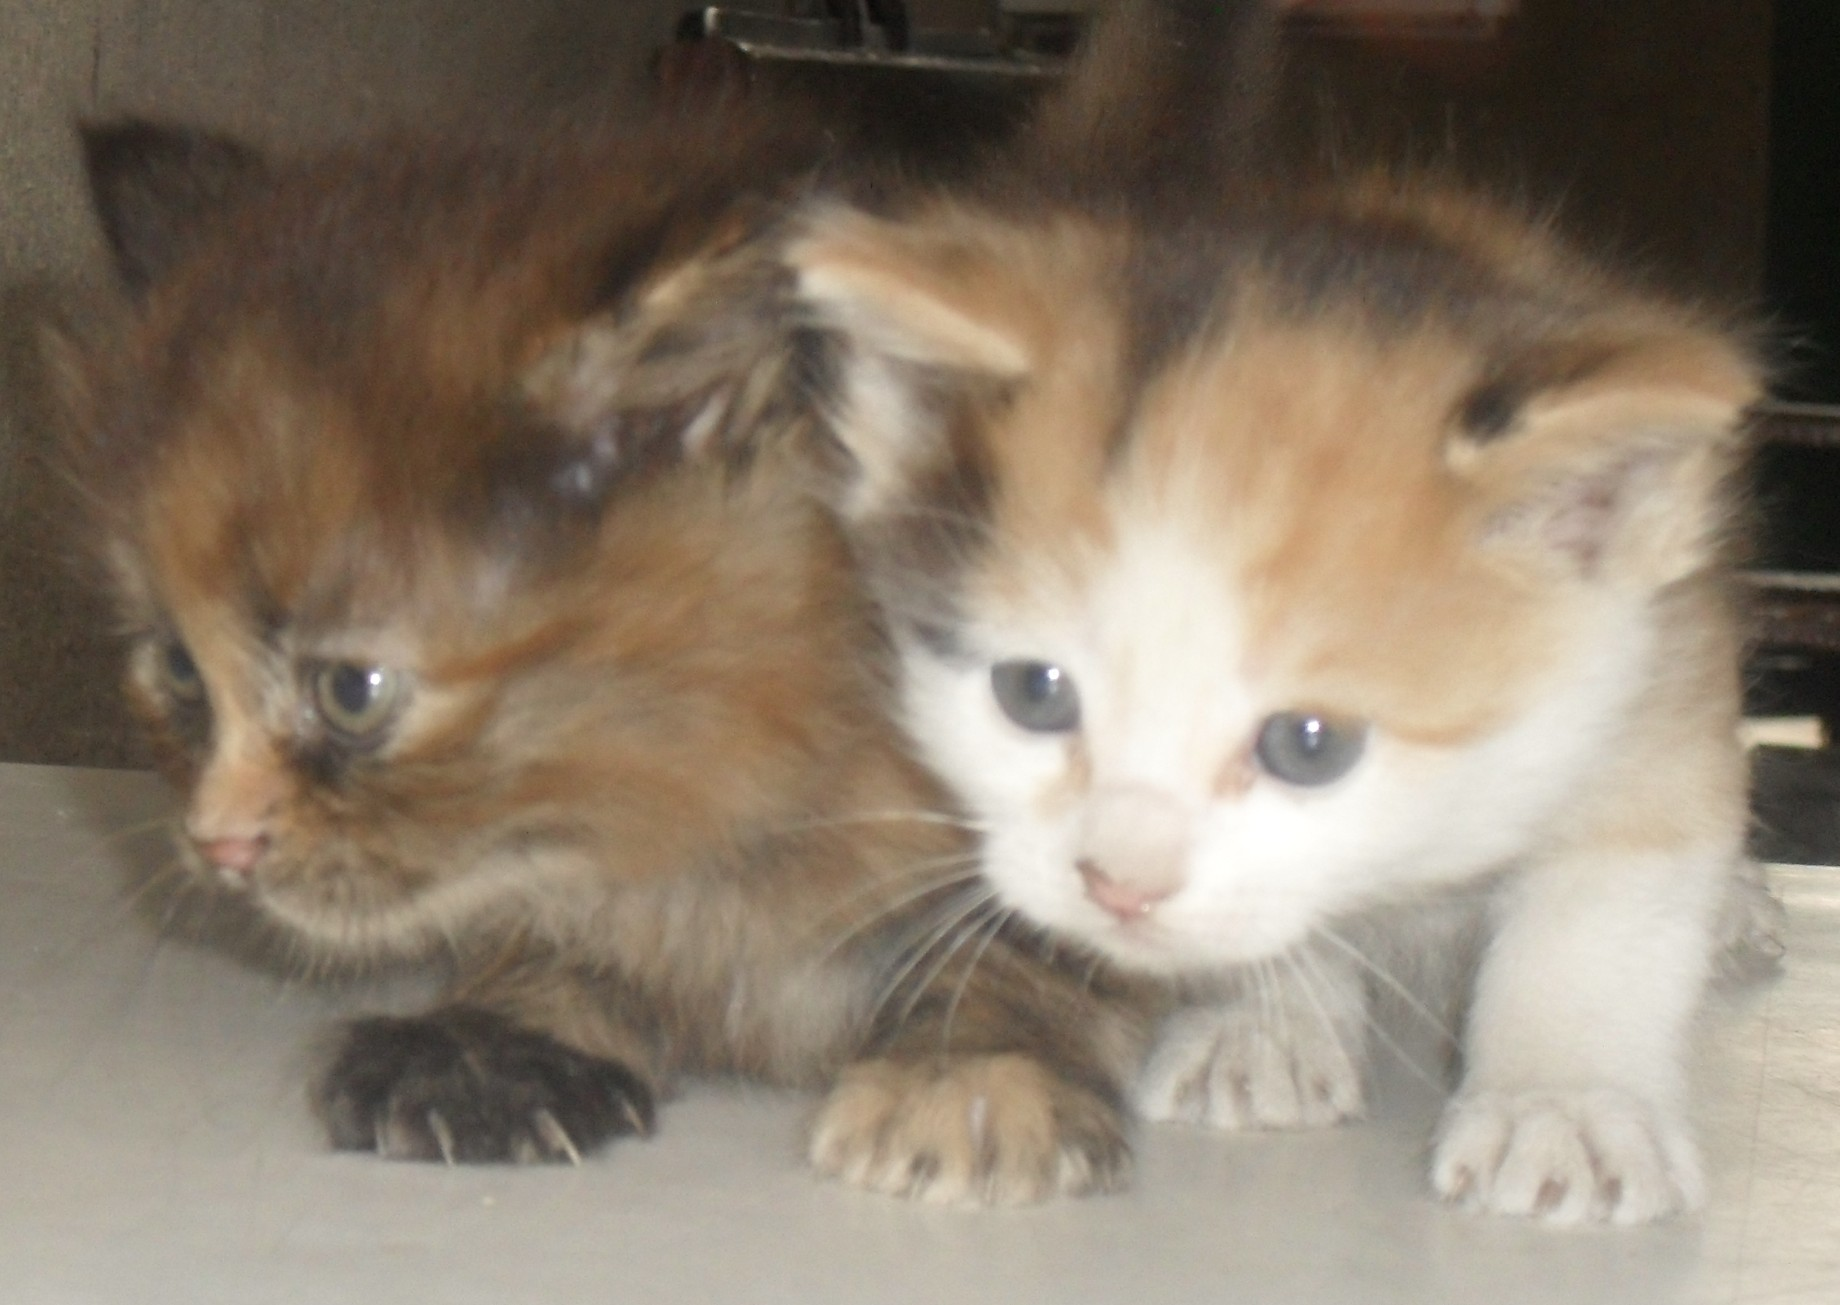
\includegraphics[keepaspectratio,width=\textwidth,height=0.75\textheight]{bild.jpg}
\caption{Ein Hund}
\label{}
\end{figure}


\end{frame}

\begin{frame}

\frametitle{Bild 2}
\label{bild2}

\begin{figure}[htbp]
\centering
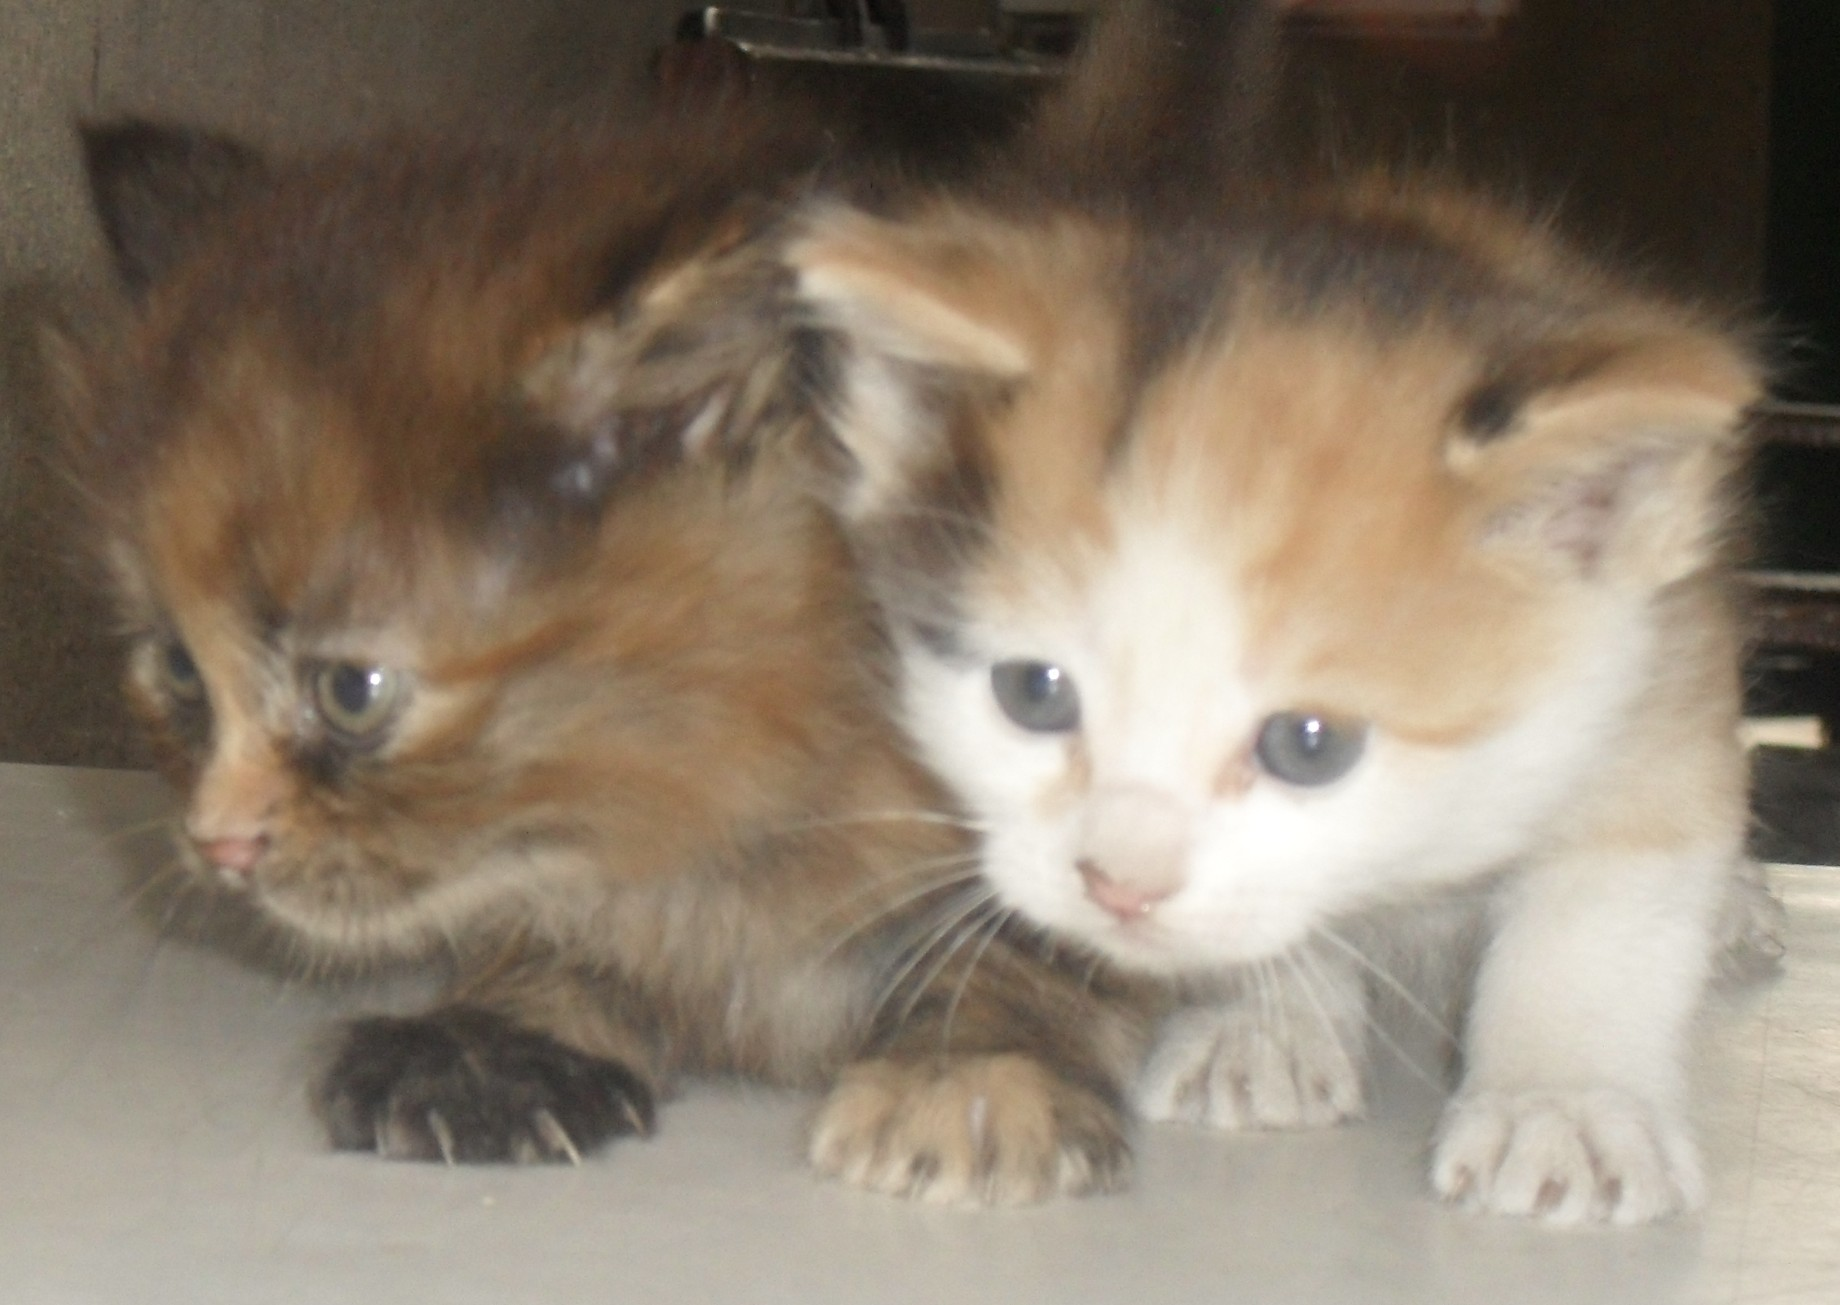
\includegraphics[keepaspectratio,width=\textwidth,height=0.75\textheight]{bild.jpg}
\caption{Zwei Katzen}
\label{}
\end{figure}


\end{frame}

\begin{frame}

\frametitle{Tabelle}
\label{tabelle}

Aus dem MultiMarkdown User’s Guide ~\citep{mmdGuide}

\begin{table}[htbp]
\begin{minipage}{\linewidth}
\setlength{\tymax}{0.5\linewidth}
\centering
\small
\caption{Prototype Table}
\label{prototypetable}
\begin{tabulary}{\textwidth}{@{}LCR@{}} \toprule
&\multicolumn{2}{c}{Grouping}\\
First Header&Second Header&Third Header\\
\midrule
Content&\multicolumn{2}{c}{\emph{Long Cell}}\\
Content&\textbf{Cell}&Cell\\

\midrule
New section&More&Data\\
And more&\multicolumn{2}{c}{And more}\\

\bottomrule

\end{tabulary}
\end{minipage}
\end{table}


\end{frame}

\begin{frame}

\frametitle{Vielen Dank für die Aufmerksamkeit!}
\label{vielendankfrdieaufmerksamkeit}

\textbf{Fragen?}

\end{frame}

\part{Bibliography}
\begin{frame}[allowframebreaks]
\frametitle{Bibliography}
\def\newblock{}
\begin{thebibliography}{0}
\bibitem{Doe}
John Doe, \emph{Ein Super Tolles Buch.} - München, 2003


\bibitem{Johnson}
John Johnson, \emph{Einfach tolles Buch.} - Berlin, 2004


\bibitem{mmdGuide}
http:/\slash fletcherpenney.net\slash multimarkdown\slash


\end{thebibliography}
\end{frame}

\mode<all>
%
%	MultiMarkdown beamer class footer file
%

% Back Matter
\if@mainmatter
\backmatter
\fi

\ifx\bibliocommand\undefined
\else
	\part{Literatur}
	\begin{frame}[allowframebreaks]
	\frametitle{Quellen}
	\bibliographystyle{\bibliostyle}
	\def\newblock{}
	\bibliocommand
	\end{frame}
\fi


\end{document}\mode*
